\begin{figure}[H]
    \centering
    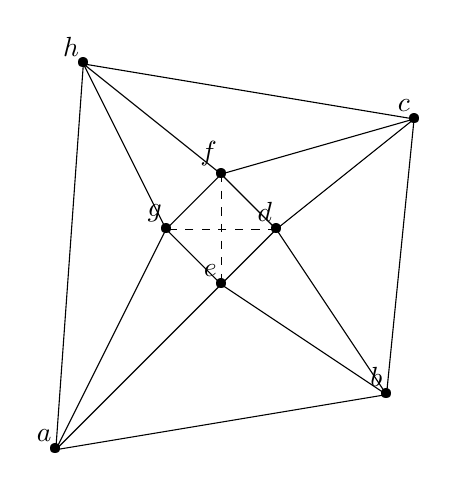
\begin{tikzpicture}[scale=0.7]
        \node[label={[label distance = -3mm]160:$a$}] at (-3, -4) {\textbullet};
        \node[label={[label distance = -3mm]160:$b$}] at (3.0, -3) {\textbullet};
        \node[label={[label distance = -3mm]160:$c$}] at (3.5, 2) {\textbullet};
        \node[label={[label distance = -3mm]160:$d$}] at (1.0, 0.0) {\textbullet};
        \node[label={[label distance = -3mm]160:$e$}] at (0, -1) {\textbullet};
        \node[label={[label distance = -3mm]160:$f$}] at (0.0, 1) {\textbullet};
        \node[label={[label distance = -3mm]160:$g$}] at (-1, 0) {\textbullet};
        \node[label={[label distance = -3mm]160:$h$}] at (-2.5, 3) {\textbullet};
        \draw (-3, -4) -- (3.0, -3);
        \draw (1.0, 0.0) -- (3.0, -3);
        \draw (3.5, 2) -- (3.0, -3);
        \draw (0, -1) -- (3.0, -3);
        \draw (1.0, 0.0) -- (3.5, 2);
        \draw (-3, -4) -- (0, -1);
        \draw (0, -1) -- (1.0, 0.0);
        \draw (-1, 0) -- (0, -1);
        \draw[dashed] (0.0, 1) -- (0, -1);
        \draw[dashed] (1, 0) -- (-1, 0);
        \draw (0.0, 1) -- (1.0, 0.0);
        \draw (0.0, 1) -- (3.5, 2);
        \draw (-3, -4) -- (-1, 0);
        \draw (-1, 0) -- (0.0, 1);
        \draw (-3, -4) -- (-2.5, 3);
        \draw (-2.5, 3) -- (-1, 0);
        \draw (-2.5, 3) -- (0.0, 1);
        \draw (-2.5, 3) -- (3.5, 2);

    \end{tikzpicture}
    \caption[Exemplo grafo de Delaunay e triangulação de Delaunay]{Para que o grafo de Delaunay
    seja uma triangulação é necessário adicionar uma das duas possíveis arestas tracejadas. O grafo
    de Delaunay da figura não é uma triangulação porque o diagrama de Voronoi desse conjunto de
    pontos tem um vértice de grau $4$.
    }\label{fig:delaunay:grafo-vs-triangulacao}
\end{figure}